\documentclass{article}
\usepackage[utf8]{inputenc}
\setlength{\parskip}{5pt} % esp. entre parrafos
\setlength{\parindent}{0pt} % esp. al inicio de un parrafo
\usepackage{listings} % listings
\usepackage{color} %colores
\usepackage{amsmath} % mates
\usepackage[sort&compress,numbers]{natbib} % referencias
\usepackage{url} % que las URLs se vean lindos
\usepackage[top=15mm,left=20mm,right=20mm,bottom=25mm]{geometry} % margenes
\usepackage{hyperref} % ligas de URLs
\usepackage{graphicx} % poner figuras
\usepackage[spanish,es-tabla]{babel} % nombre tablas


\definecolor{mypink}{rgb}{0.976, 0.462, 0.847}
\definecolor{mygray}{rgb}{0.976, 0.980, 0.980}
\definecolor{myblue}{rgb}{0.258, 0.682, 1}
\definecolor{mypink2}{rgb}{0.525, 0.054, 0.4}
\lstset{ 
  backgroundcolor=\color{mygray},
  commentstyle=\color{myblue},
  keywordstyle=\color{mypink}, 
  numberstyle=\tiny\color{mypink}
  stringstyle=\color{mypink2}, 
  breaklines=true,
}

\title{Tarea 4}
\author{Eduardo Navarro}
\date{Septiembre 2021}

\begin{document}

\maketitle

\section{Introducción}
Siguiendo las indicaciones de la clase se realizó un diagrama de voronoi al cual le aplicamos pruebas estadísticas para ver el impacto de la profundidad a la que puede llegar en relación a las semillas.

\section{Desarrollo}
Con las instrucciones de la tarea \cite{twitchsimu} se prosiguió a formar los diagramas para la posterior recolección de los datos modificando el código proporcionado en \cite{voronoi} para la obtención de estos mismos. se añadió un \texttt{for} para variar las semillas y se analizó la matriz obtenida exportando los archivos a un \texttt{.xlsx}. 

\begin{lstlisting} [language=R, caption= Código para la obtención del número de semillas y exportación.]

library(writexl)
library(ggplot2)
datos = data.frame()
n <-  15
for (k in c(5, 10, 15)) {...
return(grieta)
}
...
manhattanm <- foreach(r = 1:1, .combine=c) %dopar% propaga(r)
manhattanm
datos = rbind(datos, manhattanm)
write_xlsx(datos, "tarea4datos.xlsx")
\end{lstlisting}

Con los datos obtenidos se obtuvo la tabla \ref{tabla1}.
\newpage

\begin{table}
\centering
\caption{Datos de máximas distancias obtenidas a diferentes semillas}
\label{tabla1}
\begin{tabular}{|l|r|r|r|}
\hline
\multicolumn{1}{|c|}{\textbf{rep}} & \multicolumn{1}{c|}{\textbf{5}} & \multicolumn{1}{c|}{\textbf{10}} & \multicolumn{1}{c|}{\textbf{15}} \\ \hline
1 & 2 & 8 & 5 \\ \hline
2 & 8 & 3 & 4 \\ \hline
3 & 2 & 8 & 9 \\ \hline
4 & 8 & 4 & 4 \\ \hline
5 & 8 & 9 & 3 \\ \hline
6 & 2 & 4 & 3 \\ \hline
7 & 3 & 8 & 9 \\ \hline
8 & 8 & 3 & 5 \\ \hline
9 & 3 & 8 & 4 \\ \hline
10 & 3 & 9 & 3 \\ \hline
11 & 8 & 4 & 9 \\ \hline
12 & 8 & 3 & 9 \\ \hline
13 & 3 & 3 & 4 \\ \hline
14 & 2 & 4 & 5 \\ \hline
15 & 3 & 4 & 3 \\ \hline
\end{tabular}
\end{table}

Con los datos de la tabla \ref{tabla1} se consiguió la gráfica \ref{grafica1} donde podemos observar las distancias y el efecto de las semillas en la distribución

\begin{figure} [h!]% figura
\renewcommand{\figurename}{Gráfica}
    \centering
    \caption{Distancia mayor obtenida a diferentes semillas}
    \label{grafica1}
    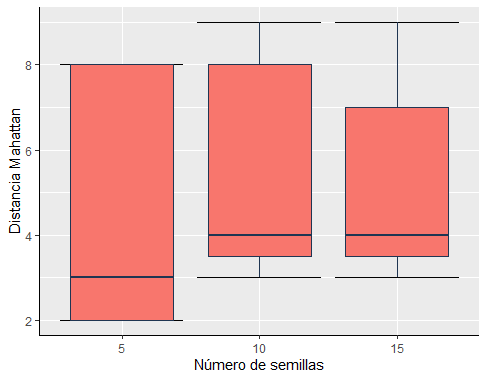
\includegraphics[width=120mm]{grafica1.png} % archivo
\end{figure}

A los datos de la tabla \ref{tabla1} se les hicieron las pruebas estadísticas de Shapiro–Wilk \cite{shapiro} y en base a los resultados obtenidos se realizó la prueba de Kruskal-Wallis \cite{Kruskall}

\begin{table}[h!]
\centering
\caption{Resultados de la prueba Shapiro–Wilk}
\label{tabla2}
\begin{tabular}{|l|r|r|}
\hline
semillas & \multicolumn{1}{l|}{w} & \multicolumn{1}{l|}{p} \\ \hline
5 & 0.70075 & 0.000253 \\ \hline
10 & 0.77555 & 0.001816 \\ \hline
15 & 0.76464 & 0.001339 \\ \hline
\end{tabular}
\end{table}


\begin{table}
\centering
\caption{Resultados de la prueba Kruskal-Wallis}
\label{tabla3}
\begin{tabular}{|l|l|}
\hline
H(2) & p-value \\ \hline
\multicolumn{1}{|r|}{3.2546} & \multicolumn{1}{r|}{0.1965} \\ \hline
\end{tabular}
\end{table}

\begin{lstlisting} [language=R, caption= Código de las pruebas estadísticas realizadas.]

#Shapiro Wilk
  lshap = lapply(tarea4datos, shapiro.test)
  lshap[[1]]
  lshap = lapply(tarea4datos, shapiro.test)
  lshap[[2]]
  lshap = lapply(tarea4datos, shapiro.test)
  lshap[[3]]
 
#Kruskal Wallis
cinco<- c(2, 8, 2, 8, 8, 2, 3, 8, 3, 3, 8, 8, 3, 2, 3)
diez<- c(8, 3, 8, 4, 9, 4, 8, 3, 8, 9, 4, 3, 3, 4, 4)
quince<- c(5, 4, 9, 4, 3, 3, 9, 5, 4, 3, 9, 9, 4, 5, 3)
  
kruskal.test(list(cinco, diez, quince))
\end{lstlisting}

\section{Conclusiones}
Al obtenerse una p menor a 0.05 en la prueba de Shapiro-Wilk se tiene que los datos no vienen de una distribución normal. Esto puede deberse a la diversa cantidad de caminos por los que la grieta se va formando en relación a la distancia máxima alcanzada. Lo mismo para la prueba de Kruskal Wallis donde la p es pequeña y no podemos rechazar la hipótesis nula donde las medianas son iguales. De forma general podemos concluir que hay más caminos formados mientras más semillas haya, por lo tanto; se crean más caminos para acercarnos, pero de la misma forma para alejarnos.

\bibliography{referencias}
\bibliographystyle{plainnat}
\end{document}
